\chapter{Trees}

Trees are one of the most versatile and widely used data structures in computer science. A tree is a hierarchical data structure consisting of nodes, where each node has a value and a set of references to its child nodes. The node at the top of the hierarchy is called the root, and nodes with the same parent are called siblings.

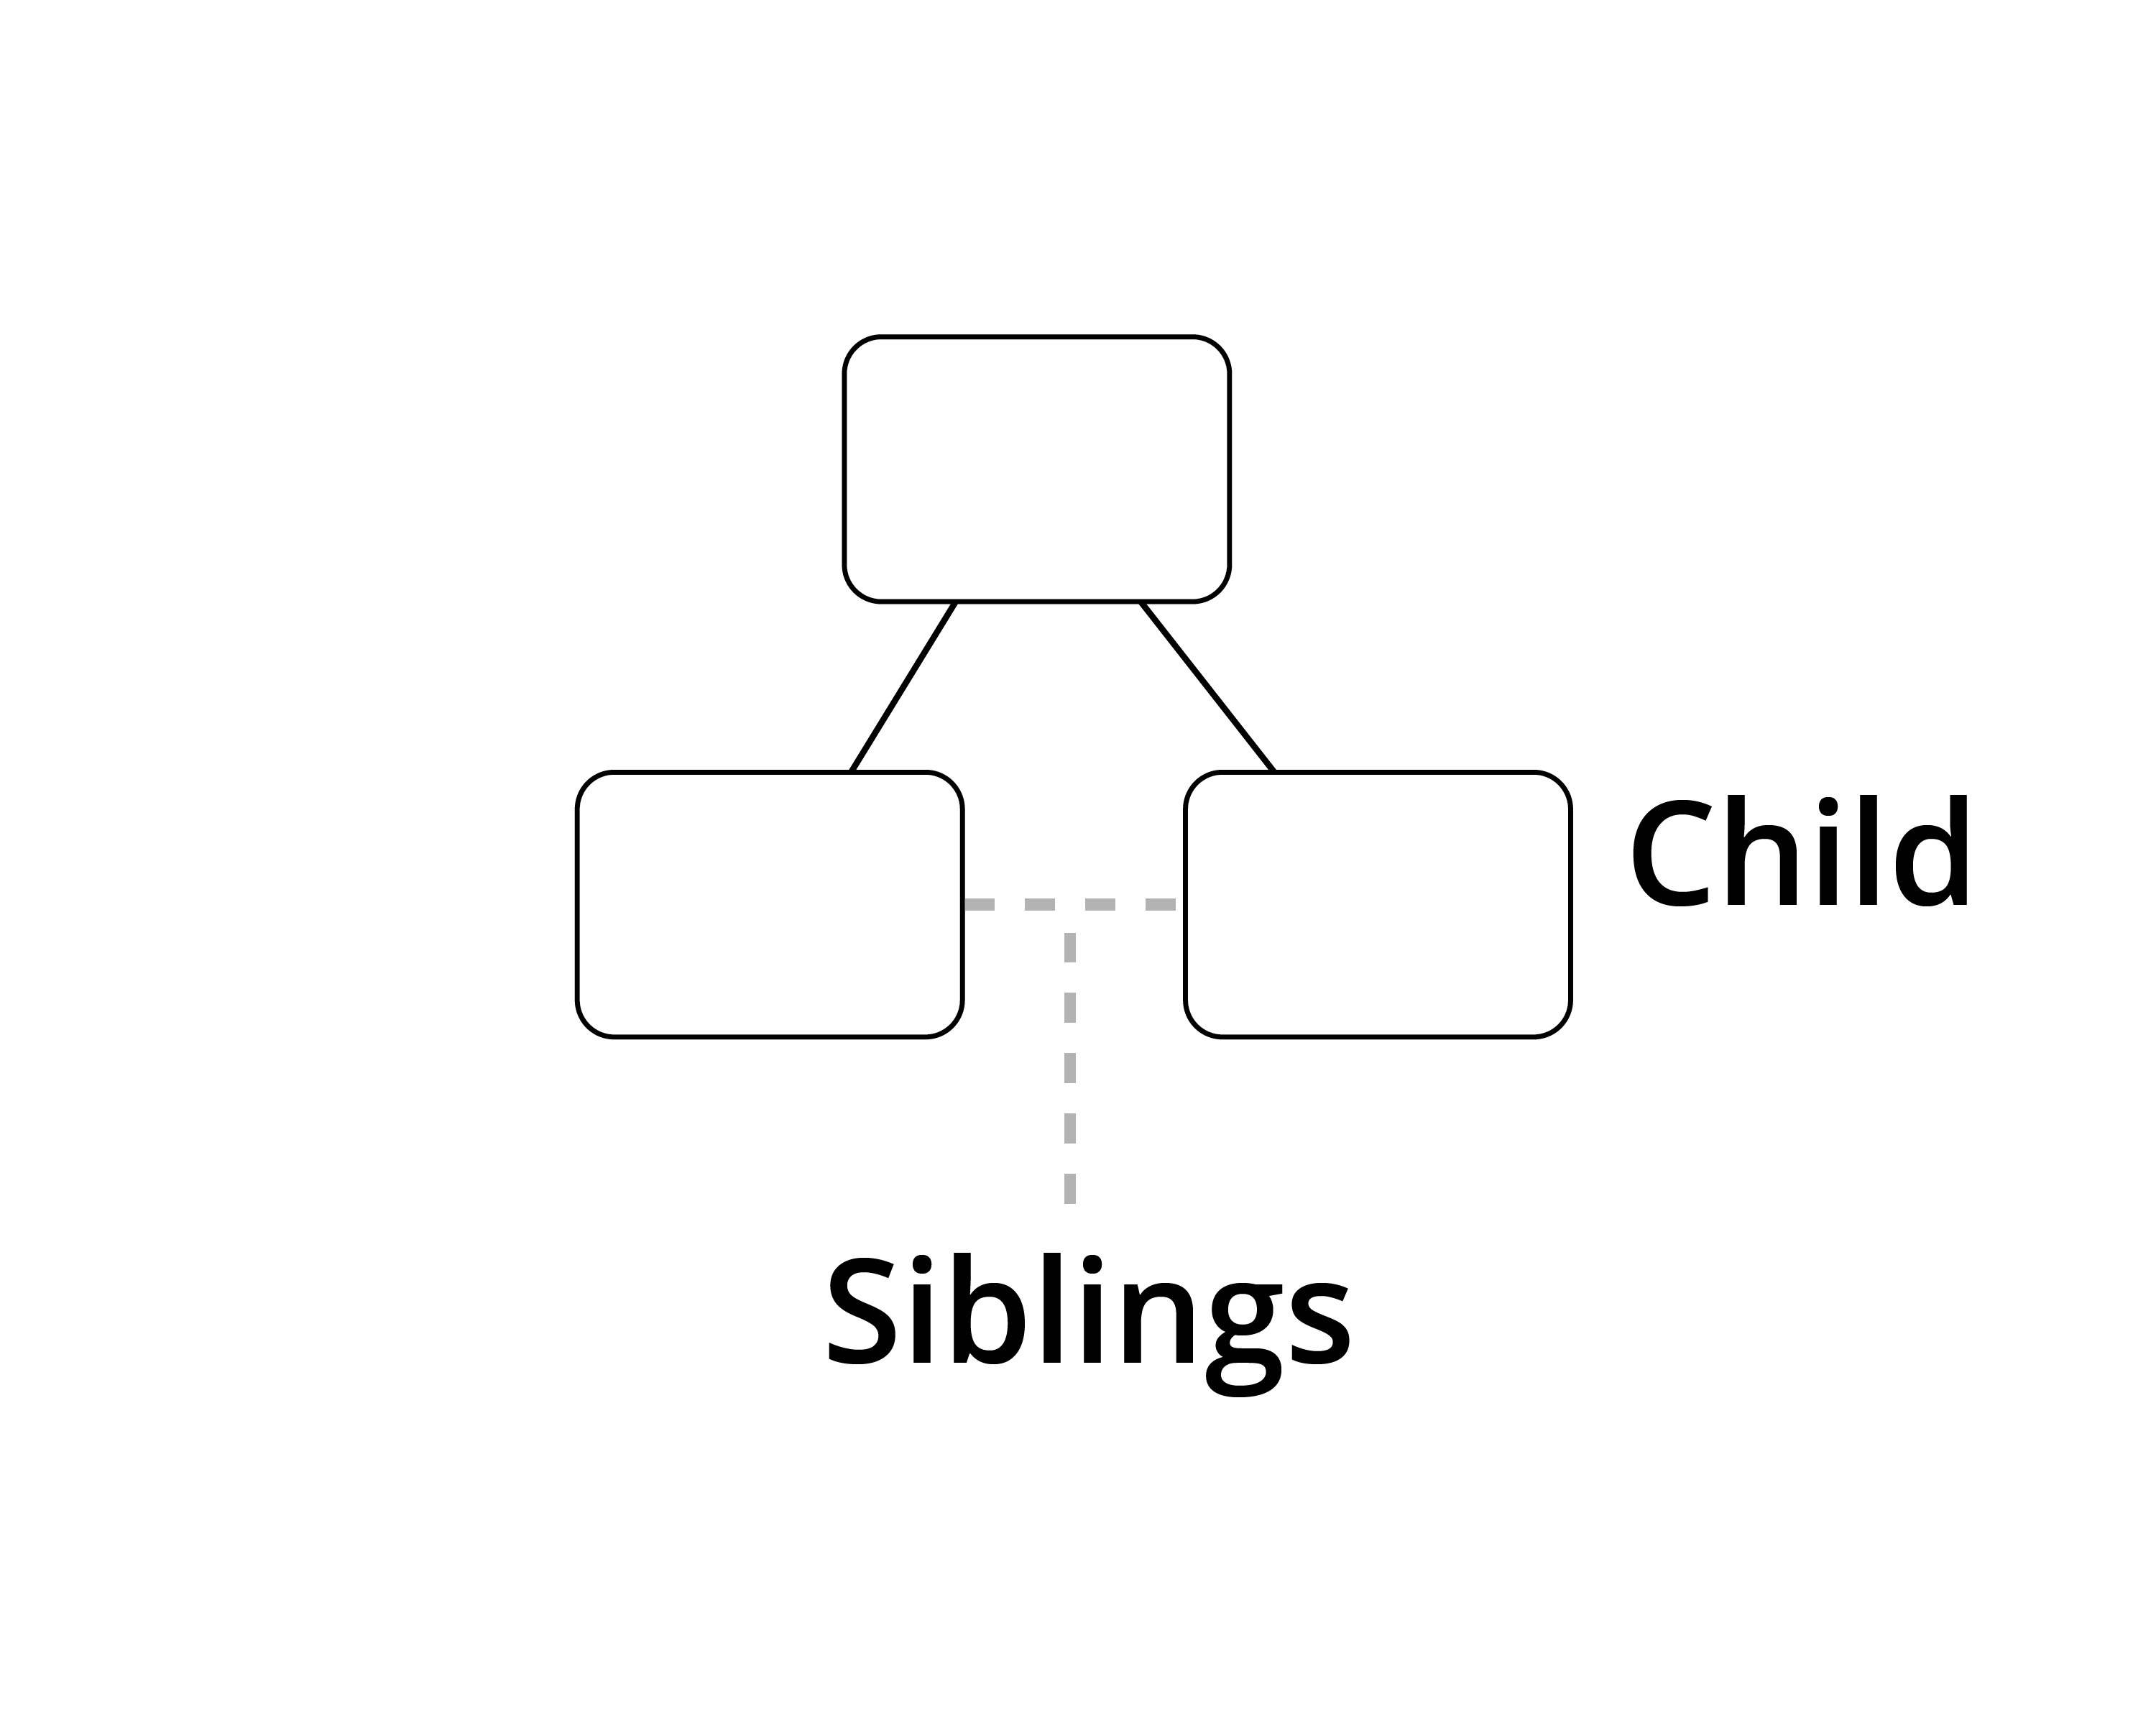
\includegraphics[width=0.75\textwidth]{parentChild.png}

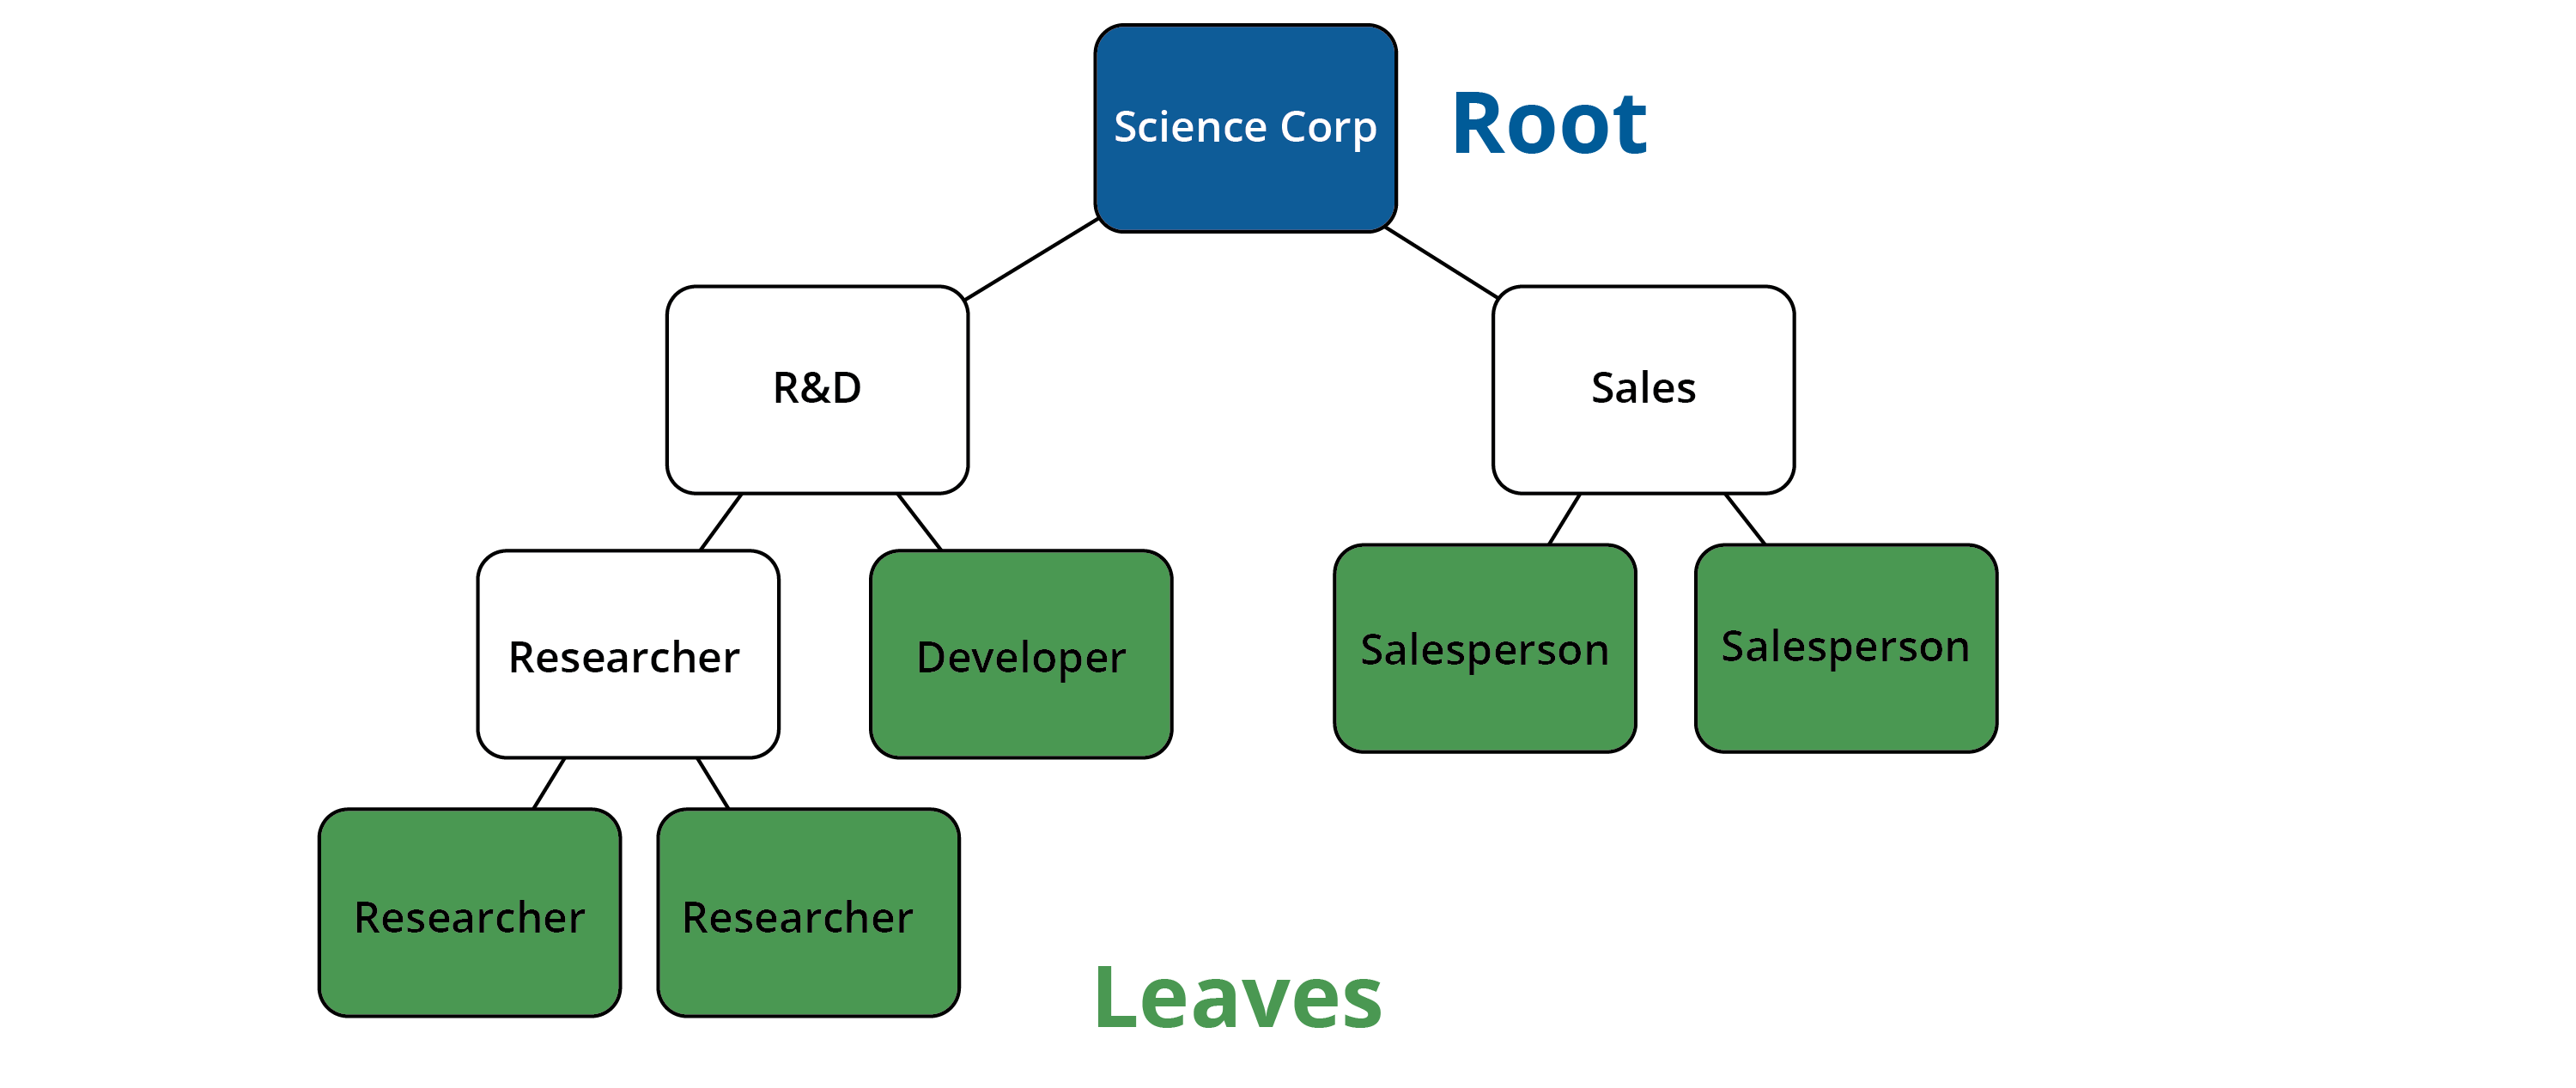
\includegraphics[width=0.75\textwidth]{rootLeaves.png}


The power of trees comes from their ability to represent complex relationships between objects, while providing efficient operations for accessing and modifying those objects. Trees can be used to represent hierarchical relationships, to organize data for quick search and insertion, and to manage sorted lists of data, among other uses.

In this chapter, we will delve into the details of the tree data structure. We will start with the definition and properties of trees, including the key concepts of roots, nodes, children, siblings, leaves, and levels. We will then introduce binary trees, a specific type of tree where each node has at most two children, which are referred to as the left child and the right child.

We will explore the various ways to traverse a tree, including depth-first and breadth-first traversals, and discuss the applications and efficiencies of these methods. We will then cover binary search trees, a variant of binary trees that allows for fast lookup, addition, and removal of items.

Then, we'll take a look at balanced search trees, such as AVL trees and red-black trees, which automatically keep their height small to guarantee logarithmic time complexity in the worst case for search, insert, and delete operations.

Finally, we will explore more advanced topics such as B-trees, tries, and suffix trees, which have applications in databases, file systems, and string algorithms.

By the end of this chapter, you will have a deep understanding of the tree data structure, its variants, and their uses. Armed with this knowledge, you'll be able to choose the right tree structure for your data and implement it effectively in your software.

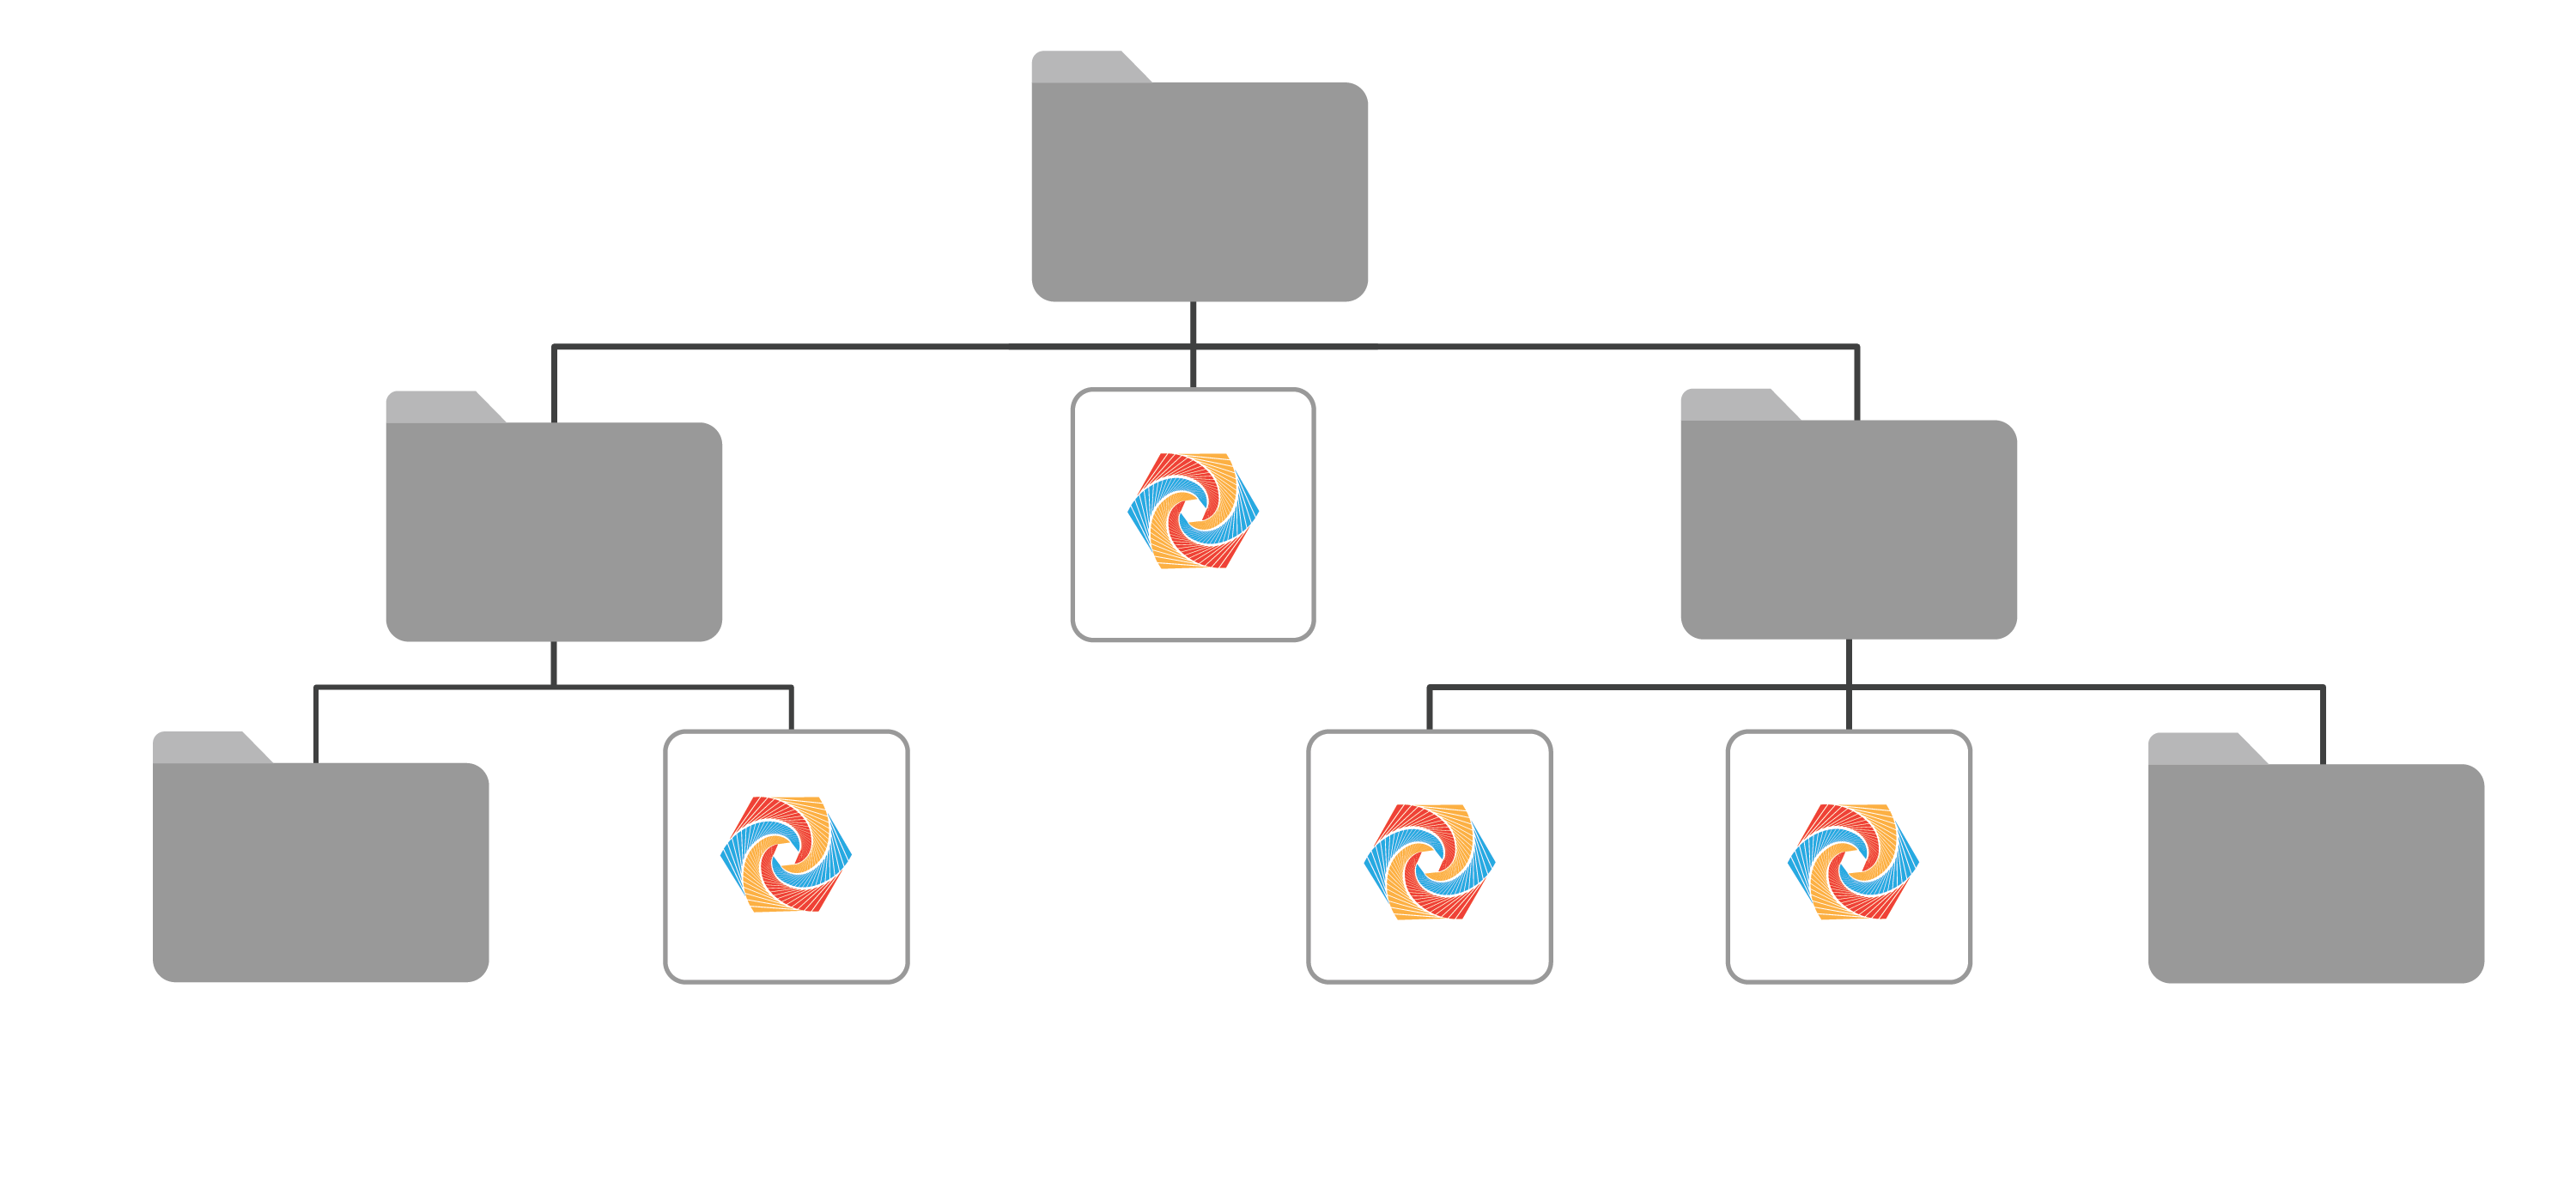
\includegraphics[width=1\textwidth]{fileStructure.png}


